\documentclass[12pt, letterpaper]{article}
\usepackage{graphicx} %LaTeX package to import graphics
\usepackage[obeyspaces]{url}

\graphicspath{{images/}} %configuring the graphicx package

\title{
    
\includegraphics[scale=0.5]{unibalogo.jpg}~\\[1cm]
    \textbf{Sviluppo di un contatore elettrico intelligente}
}
\author{Stefano Antonio Labianca}

\date{22 Gennaio 2024}
\renewcommand*\contentsname{Tabella dei contenuti}
\renewcommand{\figurename}{Figura}

\begin{document}

\maketitle


\textbf{matricola: } 758364
\hfill
\textbf{email: } s.labianca10@studenti.uniba.it

\par\noindent\rule{\textwidth}{0.4pt}~\\[5cm]

\tableofcontents ~\\[5cm]

\section{Introduzione}

Nell'arco della nostra giornata, usiamo diversi dispositivi elettronici e,
alle volte, anche per diverse ore della giornata o addirittura per tutto
il giorno. \\ \break
Per chi abita nelle zone di campagna, o in abitazioni singole, usare molti
dispositivi elettronici contemporaneamente, specialmente se hanno alti consumi o
possiedono una classe energetica bassa, fa scattare il salvavita.

\subsection{Dispositivo salvavita}

Il "salvavita", o più propriamente detto interruttore differenziale, è un dispositivo
che arresta il flusso di energia elettrica dal contatore di
un'abitazione, proteggendo persone e animali. \\ \break
Questi interruttori, monitorano la differenza di corrente in entrata
e in uscita dal dispositivo e, quando la differenza di corrente in entrata e in
uscita supera una certa soglia, allora l'interruttore scatta togliendo l'alimentazione
al circuito.

\begin{figure}
    \centering
    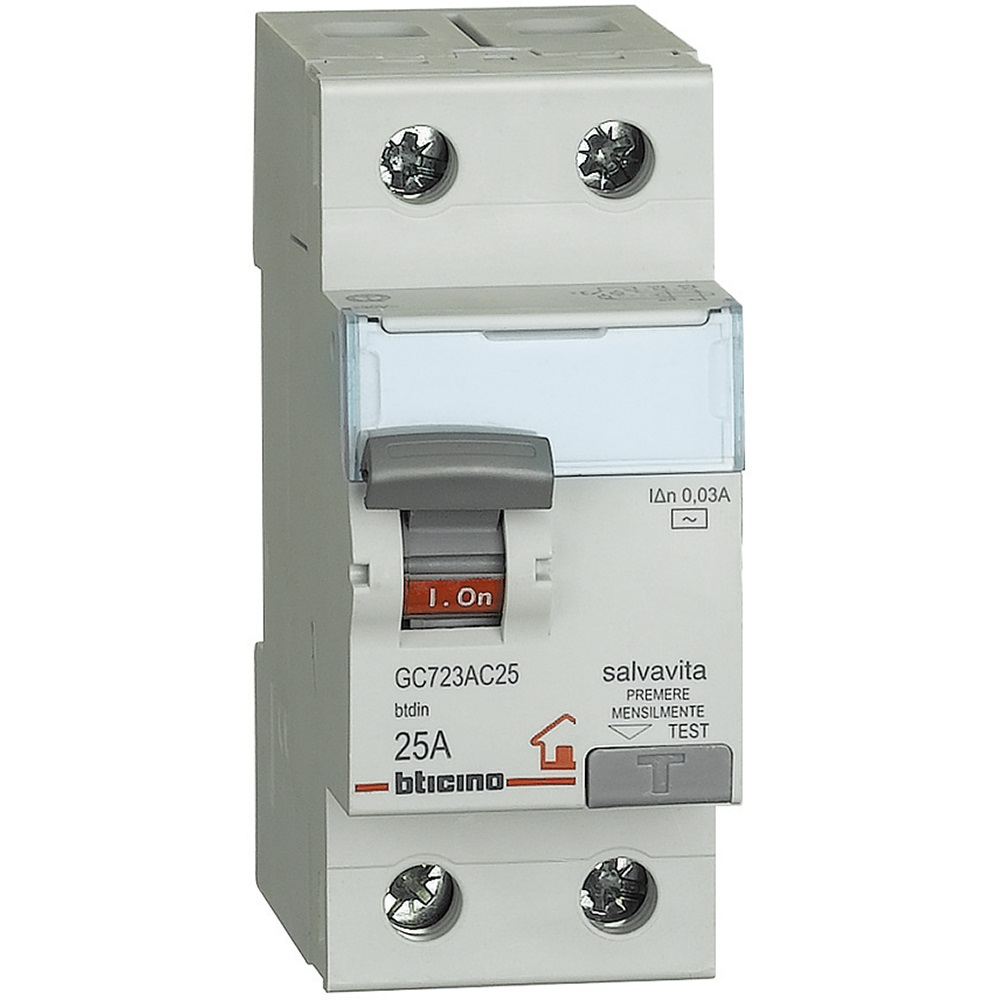
\includegraphics[scale=0.2]{interruttore-diff.jpg}
    \caption{Esempio di contatore differenziale}
\end{figure}


\subsection{Obiettivo del progetto}

Il progetto si pone l'obiettivo di sviluppare un programma in grado di svolgere
i seguenti task:

\begin{enumerate}
    \item Determinare da una lista di dispositivi, quali possono tenere accesi contemporaneamente
          senza che salti il salvavita.
    \item Tenere traccia dei dispositivi elettronici e del loro consumo in Watt.
    \item Ottenere tutti quei dispositivi che rispettano certi vincoli di consumo energetico.
\end{enumerate}

\section{Progetto}

\subsection{Struttura del progetto}

All'intero del progetto, possiamo trovare le seguenti cartelle:
\begin{itemize}
    \item \path{/appliance}: Qui è possibile trovare la classe Appliance, che definisce
          un elettrodomestico, insieme ad una serie di metodi di suppporto,
          contenuti in \path{appliances_controller.py}

    \item \path{/cli}: Troviamo una classe che incapsula tutta la logica legata agli input
          e all'output del terminale

    \item \path{/csp_problem}: Questa cartella contiene tutti i file legati all'argomento del
          CSP. \\
          Infatti è possibile trovare la rappresentazione delle variabili e dei vincoli, fatta
          rispettivamente usando le classi Variable e Constraint. \\
          Inoltre è presente anche la classe CSP usata come wrapper per rappresentare un generico
          problema di questa categoria. \\
          Infine è presenta la cartella \path{/algorithm} che contiene le realizzazioni degli
          algoritmi DFS e GAC usati per risolvere i problemi legati al CSP.

    \item \path{/knowledge_base}: Contiene una classe usata per rappresentare un Sistema Esperto.

    \item \path{/ontology}: Questa cartella contiene una classe che permette di manipolare
          l'ontologia contenuta all'intero del file \path{appliance_ontology.rdf}.

    \item \path{/test}: Contiene tutti quei file contenente vari test fatti al programma.

    \item \path{/utils}: Contiene file di utilità che facilitano alcune operazioni interne al programma.
          Per esempio, il file \path{pagination.py} viene usato per impaginare l'output del programma.
\end{itemize}

\subsection{Inizializzare il progetto}


\subsection{Avviare il progetto}



% \section{CSP}

% \section{Ontologie}


% \section{Sistema esperto}

% \section{Sviluppi futuri}

\end{document}